\documentclass{sig-alternate}
\usepackage{etoolbox}
\makeatletter
\patchcmd{\maketitle}{\@copyrightspace}{}{}{}
\makeatother

\usepackage[caption=false]{subfig}
\usepackage{verbatimbox}



\begin{document}

\title{Supervised Learning}
\subtitle{Writeup for Assignment 01 - CS 6741}

\author{
\alignauthor
Magahet Mendiola
}
\date{}

\maketitle
\begin{abstract}
An analysis of two machine learning classification problems, including an evaluation of various learning algorithms performance and behavior on the datasets.
\end{abstract}
 

%a description of your classification problems, and why you feel that they are interesting. Think hard about this. To be at all interesting the problems should be non-trivial on the one hand, but capable of admitting comparisons and analysis of the various algorithms on the other.

\section{Data}

Two classification datasets have been chosen based on the following criteria: Each dataset includes a minimum of 3,000 instances to insure sufficient data to evaluate each learning algorithm. Test sets were created by taking a uniform random sample of 33\% of the original instances without replacement. The remaining 66\% were then used as a training superset. Smaller subsets were pulled from this partition as needed.


\section{Classification - Mushrooms}

The first dataset is titled, Mushroom \cite{Bache+Lichman:2013} and was chosen from the UCI ML Repository. The classification task for this dataset is to determine whether a given mushroom is edible or poisonous based on the specimen's physical attributes. There are 22 recorded attributes which describe the physical appearance and olfactory perception of each sample. A full description of attributes can be found at http://archive.ics.uci.edu/ml/datasets/Mushroom.

This dataset allows for experimentation of various learning algorithms against attributes with only discrete values. The recorded attributes also require minimal domain knowledge to interpret, which reduces complexity in conceptualizing relationships and evaluating each learner's behavior.


\subsection{Attribute characteristics}

By examining the value distributions as seen in Figure~\ref{ag-data-viz}, we first observe that the two classifications are fairly evenly distributed (48\% edible, 52\% poisonous). This allows for the evaluation of learning algorithm accuracy based on the percentage of classification mistakes made by the model on our test set. This metric will not be unduly weighted by a greater occurrence of one of the classes. It is worth considering the use case for such a classification task though. For example, if this model were to be used to decide whether to serve a given mushroom to a class full of students, we would prefer a hypothesis that favored misclassification of edible over that of poisonous. This idea will be examined while exploring the test results.

Each attribute includes a finite and limited set of values (min: 2, max:12). This indicates that information gain would provide a suitable metric for decision tree attribute selection, as the variance in value ranges is not significant and, similar to our reasoning for class distribution, we will not need to account for attributes with greater than average ranges of values.

With all the attributes taking discrete (nominal) values, we will be somewhat constrained in learning algorithms options. For example, neural network network input nodes will need to be setup for each attribute value pair; separating them into binary attributes for each value. Similarly, nominal attributes will limit the capabilities of SVM. Non-linear kernels will not be effective in increasing the, already linearity separable, feature space. The behavior of k-nn will also be constrained as well. Distance metrics for such attributes will either be simplistic (testing for exact matches) or less intuitive than measuring euclidean distance.

\begin{figure}[!htbp]
    \centering
    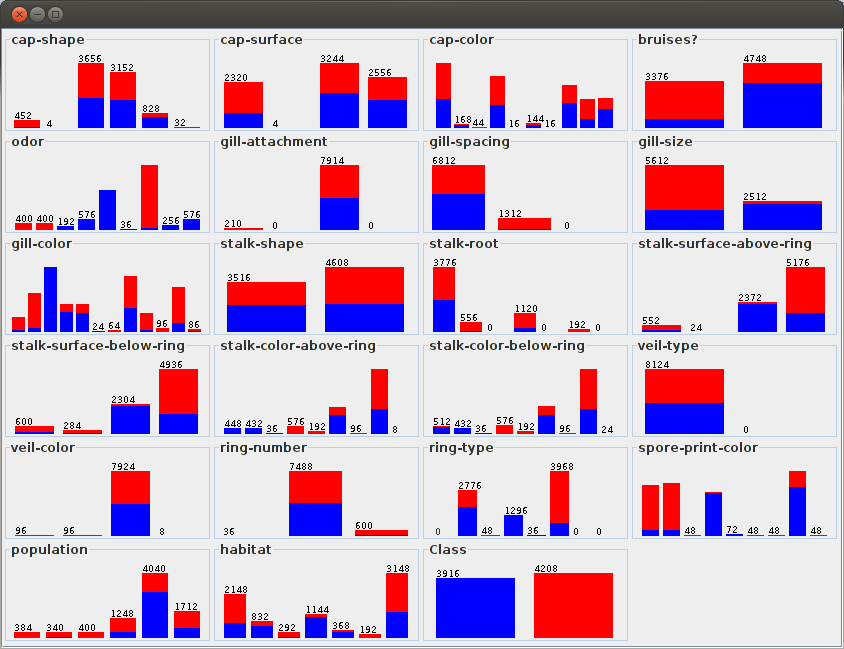
\includegraphics[width=3in]{data/agaricus-lepiota/ag-data-viz.png}
    \caption{mushroom attribute distribution and classification \label{ag-data-viz}}
\end{figure} 

It can also be observed visually that a number of attributes provide clear separability between the target classes. This supports the intuition that this set of attributes does have some functional relationship to the classes. In fact it appears, from the figure, that the attribute ``odor'' by itself could provide a fairly clear indicator of how a sample should be classified. ``Spore-print-color'' appears to provide decent class separation as well. It can be predicted that these attributes will be heavily weighted during the attribute selection or weighting process.

\subsection{Algorithm Evaluations}
%the training and testing error rates you obtained running the various learning algorithms on your problems. At the very least you should include graphs that show performance on both training and test data as a function of training size (note that this implies that you need to design a classification problem that has more than a trivial amount of data) and--for the algorithms that are iterative--training times.

Each leaning algorithm has been applied to the training data with the same procedure. As described earlier, a subset of data was partitioned and preserved as a training set. The remain instances were then sample from to create smaller training sets for use in evaluating each learning algorithms' performance and behavior.


\subsubsection{Learning Curves}

Evaluation began by choosing conservative starting values for each learners' parameters. Then each learner was trained against a range of training set sizes between 10 and 2000 instances (increments of 10). After each training phase, the original test data (1/3 of the original dataset) was used to evaluate the learner's performance. In this case classification error was used as the performance metric. The plot in Figure~\ref{ag-error} shows each learning algorithm's results.

A number of assumptions are made for this initial evaluation. The goal of the exercise being to obtain a general intuition regarding each algorithms' performance, and not to present ideal conditions. Further parameter changes are discussed in subsequent sections of this analysis. The following describes the initial conditions for each learning algorithm.

\begin{description}
    \item[Decision Tree] Weka's open source version of the C4.5 algorithm (J48) was chosen, which uses normalized information gain ratio to select attributes. Post-pruning was done with a minimum leaf size of 2 instances a confidence factor of 0.25.
    \item[Boosting] Although it would be beneficial to compare our single iteration C4.5 to the same learner with boosting enable, unfortunately that was not possible with this dataset. As can be observed in the learning curve plots below, the training error for J48 was negligible. This caused the AdaBoost algorithm to compute a zero classification error tree in most cases. This resulted in the boosting process returning after a single decision tree is built. This result persisted even with more aggressive post-pruning parameters. In order to evaluate boosting, a weaker learner was chosen in place of C4.5. Boosting was performed on a decision stump learner, which is a simplistic decision tree algorithm that creates a single node/attribute tree.
    \item[Neural Network] A multilayer perceptron network was used with one hidden layer using a sigmoid activation function. Input nodes were created for each attribute/value pair, and 63 hidden nodes were used, which is the number of input nodes plus the number of output nodes divided by two. The algorithm performs gradient decent to adjust weights, and includes both a learning rate and a momentum factor to slow down and smooth weight changes. For this test, both terms are held static (learning rate = 0.3, momentum = 0.2).
    \item[k-NN] For the initial tests, the nearest neighbor algorithm was set to k = 1. This matches the single closest instance from the training set to determine a classification. The distance metric used is euclidean distance. The plot titles for k-NN are IBk, which is the Weka implementation of k-NN. 
    \item[SVM] SVM was run initially with a linear kernel. Both polynomial and radial basis function kernels are evaluated later. The plot title for SVM is SMO, which is Weka's implementation of SVM.
\end{description}

\begin{figure}[!htbp]
    \centering
    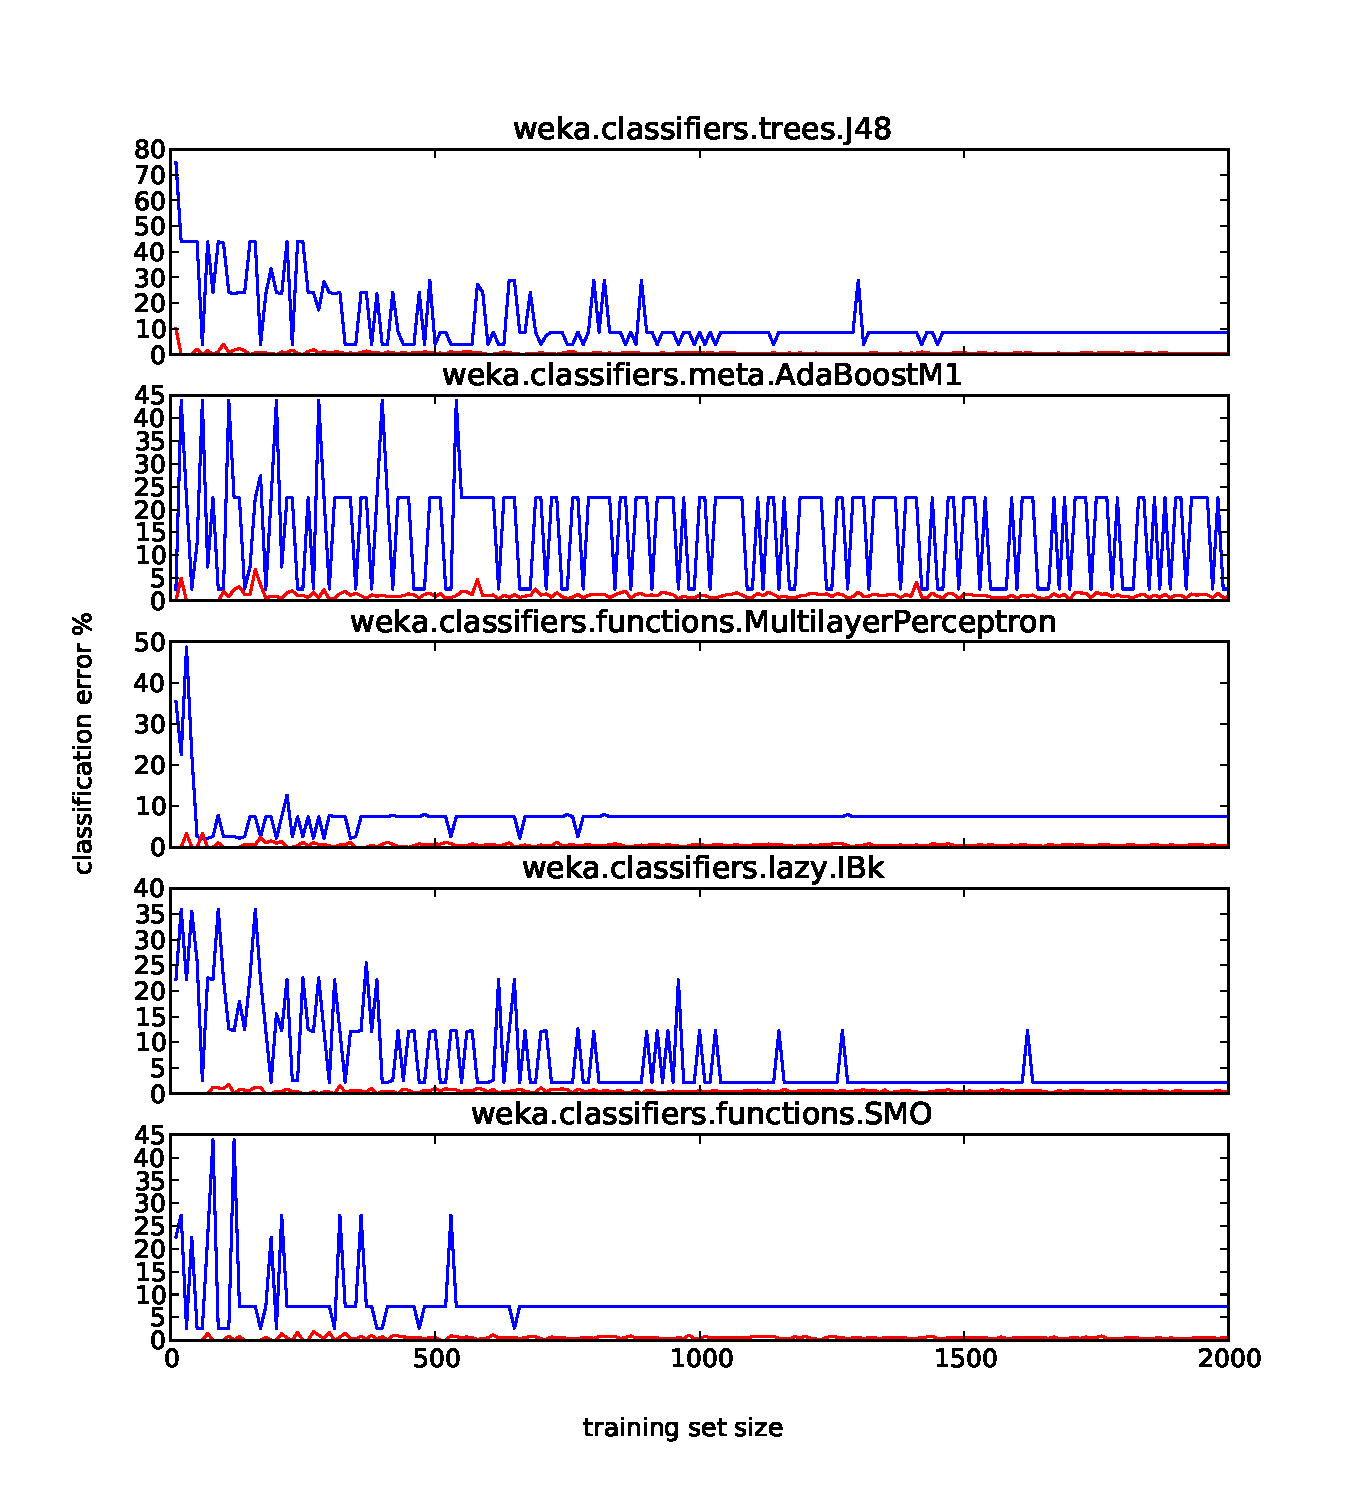
\includegraphics[width=3in]{data/agaricus-lepiota/learning-curve-10to2000/stacked-test-error.pdf}
    \caption{Mushroom - Classification Error by Training Size \label{ag-error}}
\end{figure} 

The results show training error (red lines) for every learner remain below 10\%. In all cases, except decision trees, this error was never higher than 5\% even with only 10 samples to train from. This indicates that our learners were able to converge to a hypothesis that fit the training data very well for even small sample sizes. The overall dataset seems to have a little variance and each learner is able to closely model the training data.

The test error plots also exhibit low error for most learners, with the exception of boosting. As expected, smaller training sample sizes show higher misclassification rates. The error rates quickly drop to below 10\% for training sets around 1,000 samples. Comparing each learner, we see that our perceptron network was able to reach this low level of classification error with the smallest number of training examples (~100). However, the runtime plot in Figure~\ref{ag-runtime} shows that this learner was the slowest to train by an order of magnitude. Depending on the use case, a trade-off can be made for which learner to implement.

Another interesting result is from our boosting algorithm, which struggled to reach the same level of classification error as the others. The intuition for this is that as there are certain attributes with much greater performance metric results which unduly influenced the ability of the weak learner to find suitable attributes other than those with the most influence on the classification.


\subsubsection{Training Times}

The elapsed time required for each learner to consume the training set has been plotting in Figure~\ref{ag-runtime}. Results from this data indicate that C4.5 performed well empirically. Training time for decision trees appeared to run two orders of magnitude faster than our neural network, and one order greater than SVM. The perceptron network seemed to growing linearly and remained far above any other learner. The one surprise in the results was k-NN, which seemed to take longer to train than decision trees. This may be due to the preprocessing of samples to prepare them for distance measurements, such as pre-sorting.


\begin{figure}[!htbp]
    \centering
    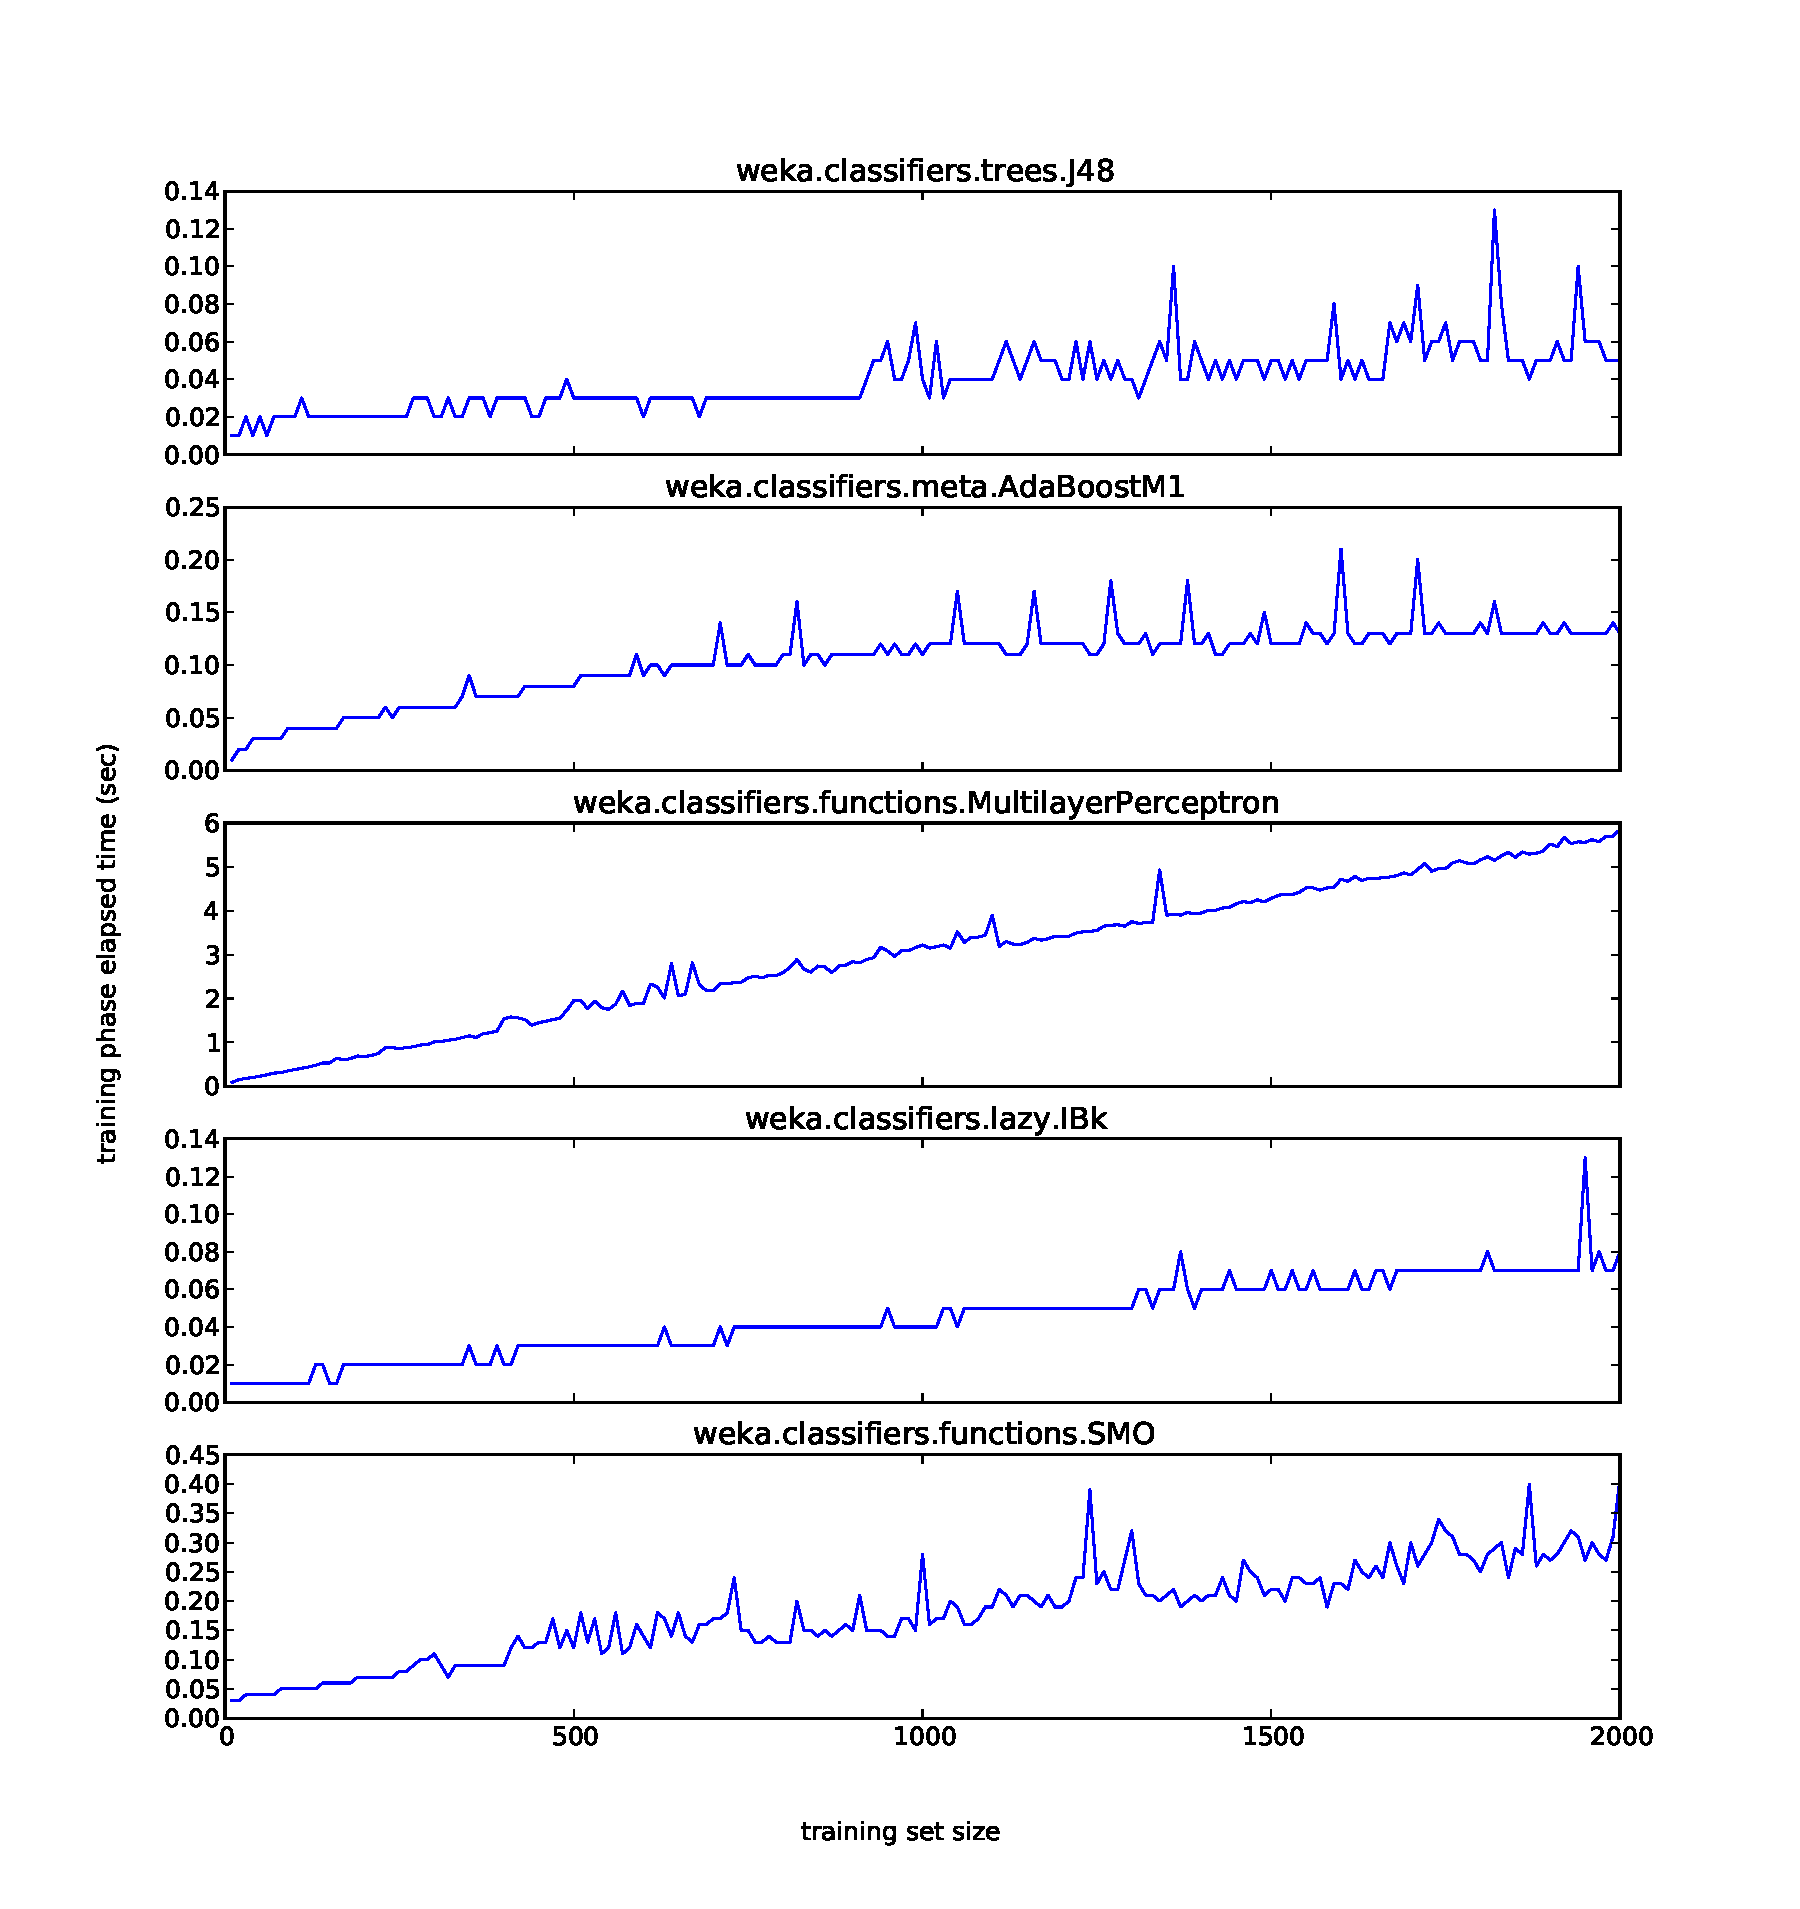
\includegraphics[width=3in]{data/agaricus-lepiota/learning-curve-10to2000/runtime.pdf}
    \caption{Mushroom - Training Time by Training Size \label{ag-runtime}}
\end{figure} 


\subsubsection{Decision Trees}
%Decision Trees. For the decision tree, you should implement or steal a decision tree algorithm. Be sure to use some form of pruning. You are not required to use information gain (for example, there is something called the GINI index that is sometimes used) to split attributes, but you should describe whatever it is that you do use.

Further experimentation into the decision tree learner was performed on subsets of the original data. As before, 1/3 of the data was partitioned for testing. The training set was then taken as 1,000 instances from the remaining set.

As a baseline, the learner was run with initial settings, which included post-pruning with a 0.25 confidence factor and a minimum leaf size of 2 instances. These settings produced the tree in Figure~\ref{dt-c025}. This tree produced no training classification error and 12\% error on the test set. The majority of training instances were classified based on two attributes, odor and stalk-shape.

The discrepancy in training and testing error indicates that the learner may be overfitting the training data. This is further supported by the small number of instances categorized by deeper leaves. To try to archive better generalize, the same process was repeated with more aggressive post-pruning parameters. The results of setting the confidence factor to 0.01 is shown in Figure~\ref{dt-c001}.

Although a negligible number of instances were miscategorized from the training set, the classification error on the test set dropped to 4\%. The resulting tree is made up of a single attribute node with nine leaves. This confirms the initial hypothesis that overfitting was occurring with the initial parameters. It can also be seen that, as expected, the odor attribute does in fact exert a great deal of influence on correct classification. To validate this further, Weka's attribute evaluator tool was used to calculate the information gain for this attribute, which came out at 0.83. This confirms further the strength of this attribute in classification.

It should be noted that Adjusting the post-pruning parameters further would have no effect on the tree, as it cannot be pruned further. When run with no post-pruning performed, the same tree is produced as with the initial settings.

\begin{verbbox}

odor = a: e (69.0)
odor = l: e (77.0)
odor = c: p (37.0)
odor = y: p (6.0)
odor = f: p (234.0)
odor = m: e (0.0)
odor = n
|   stalk-shape = e
|   |   habitat = g: p (3.0)
|   |   habitat = l
|   |   |   bruises? = t: p (3.0)
|   |   |   bruises? = f: e (4.0)
|   |   habitat = m: p (4.0)
|   |   habitat = p: e (0.0)
|   |   habitat = u: e (16.0)
|   |   habitat = w: e (18.0)
|   |   habitat = d
|   |   |   stalk-surface-above-ring = f: p (0.0)
|   |   |   stalk-surface-above-ring = y: p (0.0)
|   |   |   stalk-surface-above-ring = k: p (4.0)
|   |   |   stalk-surface-above-ring = s: e (4.0)
|   stalk-shape = t: e (468.0)
odor = p: p (51.0)
odor = s: p (2.0)

Number of Leaves  :     20

Size of the tree :  25

\end{verbbox}

\begin{figure}[!htbp]
    \centering
    \theverbbox
    \caption{c4.5 decision tree with 0.25 confidence interval \label{dt-c025}}
\end{figure}


\begin{verbbox}

odor = a: e (69.0)
odor = l: e (77.0)
odor = c: p (37.0)
odor = y: p (6.0)
odor = f: p (234.0)
odor = m: e (0.0)
odor = n: e (524.0/14.0)
odor = p: p (51.0)
odor = s: p (2.0)

Number of Leaves  :     9

Size of the tree :  10

\end{verbbox}

\begin{figure}[!htbp]
    \centering
    \theverbbox
    \caption{c4.5 decision tree with 0.01 confidence interval \label{dt-c001}}
\end{figure}

\subsection{Neural networks}
%For the neural network you should implement or steal your favorite kind of network and training algorithm. You may use networks of nodes with as many layers as you like and any activation function you see fit.

The neural network learner was able to reach a low classification error with a very small training set (around 100 instances). To evaluate this learner in greater detail, the experiment was repeated with the following conditions:

\begin{itemize}
    \item training set size was held at 1,000 instances
    \item learning rate (how much weights are changed each iteration), were varied from 0.1 to 3.0
    \item training iterations are varied between 10 and 1,000 (by 10s)
    \item number of hidden nodes are varied manually
\end{itemize}

The results from varying the learning rate and training iterations  is displayed in Figures~\ref{ag-nn-ti}~and~\ref{ag-nn-lr}. These plots show variance in the classification error for training iterations and learning rate. However, there is no discernible trend that would indicate better performance of the learner with a specific parameter value.

From examination of the attribute value distribution, and interpreting the results from the decision tree algorithm, it can be hypothesized that very few attributes have an influence on classification. Furthermore, there seems to be a direct relationship between those attributes and the class. This leads to the intuition that hidden layers in our neural network may be superfluous. It turns out, through repeating the experiment with decreasing numbers of hidden nodes, that classification error does not increase considerably. When a network with no hidden layer is trained, the error actually dropped from 7.7\% to 7.6\%. The significant advantage to this simplified network is the training time difference. The new network, with 63 fewer nodes, was able to train on the dataset in 1\% of the original time.

It is also interesting to note that the attributes identified by the decision tree algorithm as being the most relevant show the highest weights on the output nodes. This can be seen in the subset of weight outputs in Figure~\ref{ag-nn-weights}.


\begin{figure}[!htbp]
    \centering
    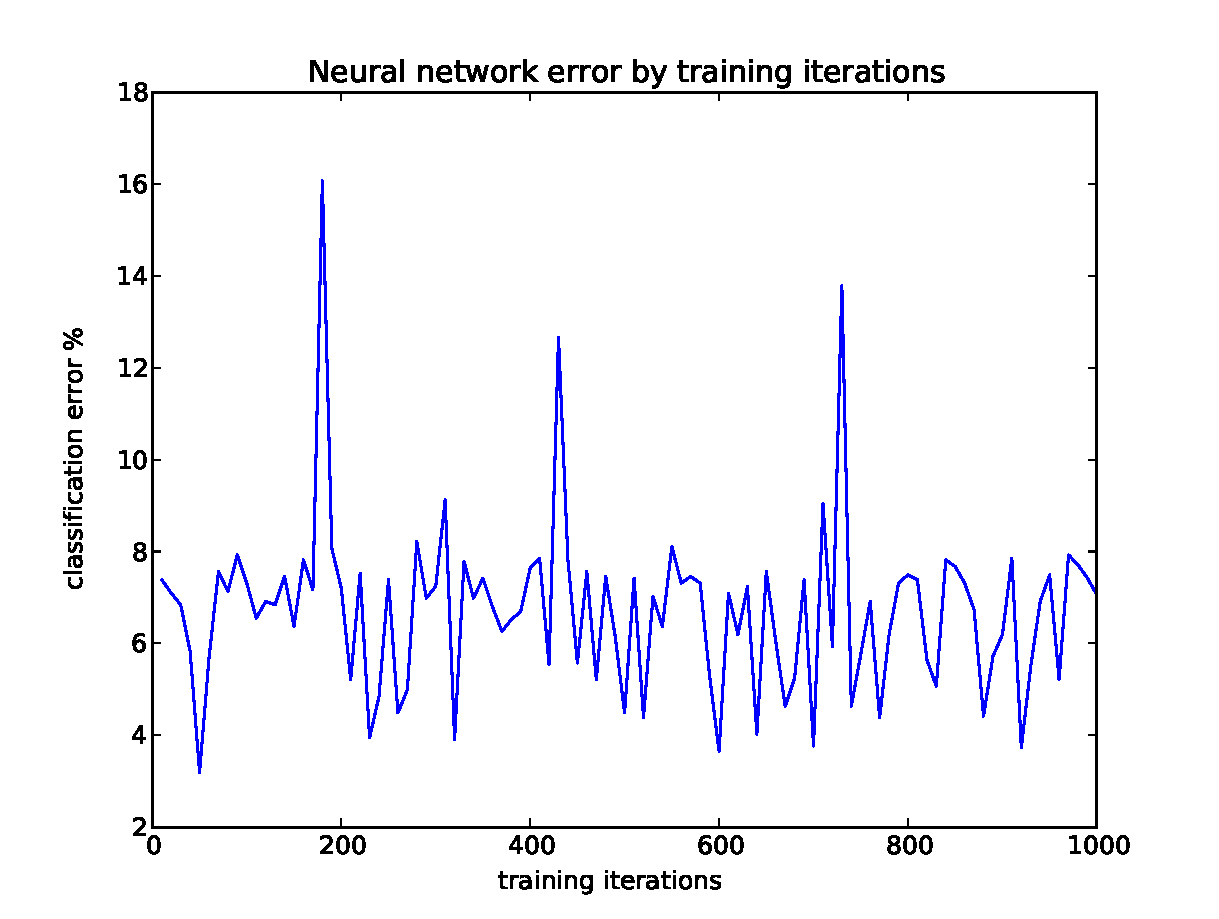
\includegraphics[width=3in]{data/agaricus-lepiota/perceptron/training-iterations.pdf}
    \caption{mushroom - neural network error by training iterations \label{ag-nn-ti}}
\end{figure} 

\begin{figure}[!htbp]
    \centering
    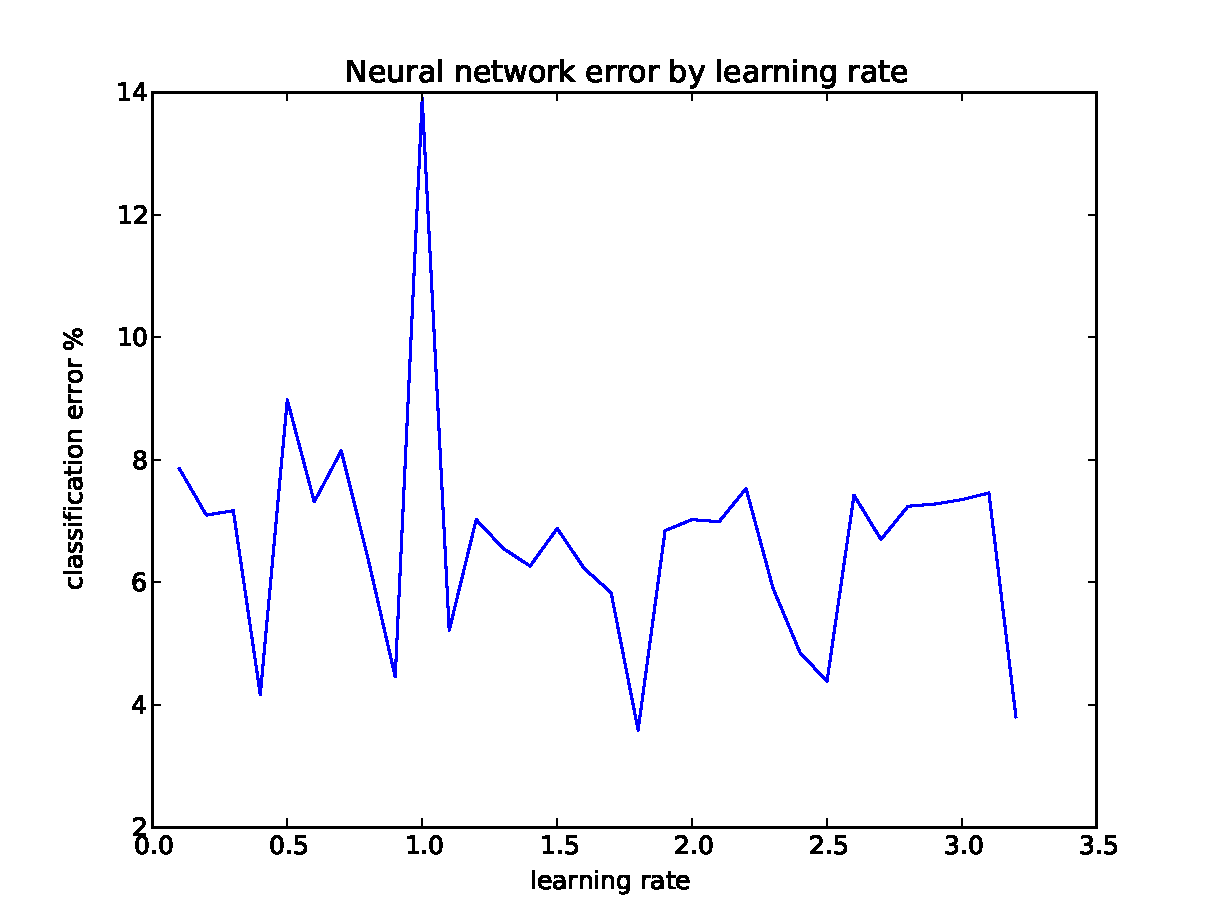
\includegraphics[width=3in]{data/agaricus-lepiota/perceptron/learning-rate.pdf}
    \caption{mushroom - neural network error by learning rate \label{ag-nn-lr}}
\end{figure} 

\begin{verbbox}
Attrib cap-color=u    0.32909165328321105
Attrib cap-color=e    0.27084200618784854
Attrib cap-color=w    -0.6781600170313064
Attrib cap-color=y    -0.0944215007903694
Attrib bruises?    -0.20164966240021834
Attrib odor=a    1.9591467769018915
Attrib odor=l    2.163249089101404
Attrib odor=c    -1.938000290279853
Attrib odor=y    -0.7210176961657636
Attrib odor=f    -1.4655475615783258
Attrib odor=m    -0.0022502391144373773
Attrib odor=n    2.249162579023187
Attrib odor=p    -2.08204828811813
Attrib odor=s    -0.2329200532370795
Attrib gill-attachment=a    -0.016241324327899875
Attrib gill-attachment=d    0.0167616393841718
Attrib gill-attachment=f    0.04167201385764717
Attrib gill-attachment=n    -0.023866806192559844
Attrib gill-spacing=c    -0.8456690489234284
Attrib gill-spacing=w    0.8125552864255976
\end{verbbox}

\begin{figure}[!htbp]
    \centering
    \theverbbox
    \caption{neural network sample output node weights \label{ag-nn-weights}}
\end{figure}


\subsection{Boosting}
%Implement a boosted version of your decision trees. As before, you will want to use some form of pruning, but presumably because you're using boosting you can afford to be much more aggressive about your pruning.

As noted earlier, the boosting algorithm continued to oscillate between high and low classification errors as the training set size increased. A follow up test was performed to see if differing boosting iterations would have an effect on the overall error. The results are shown in Figure~\ref{ag-boost-iter}. This plot shows that after around 50 training iterations, boosting began producing models with higher classification error on the test set. This indicates that overfitting begins to occur and the model is no longer able to generalize well.

\begin{figure}[!htbp]
    \centering
    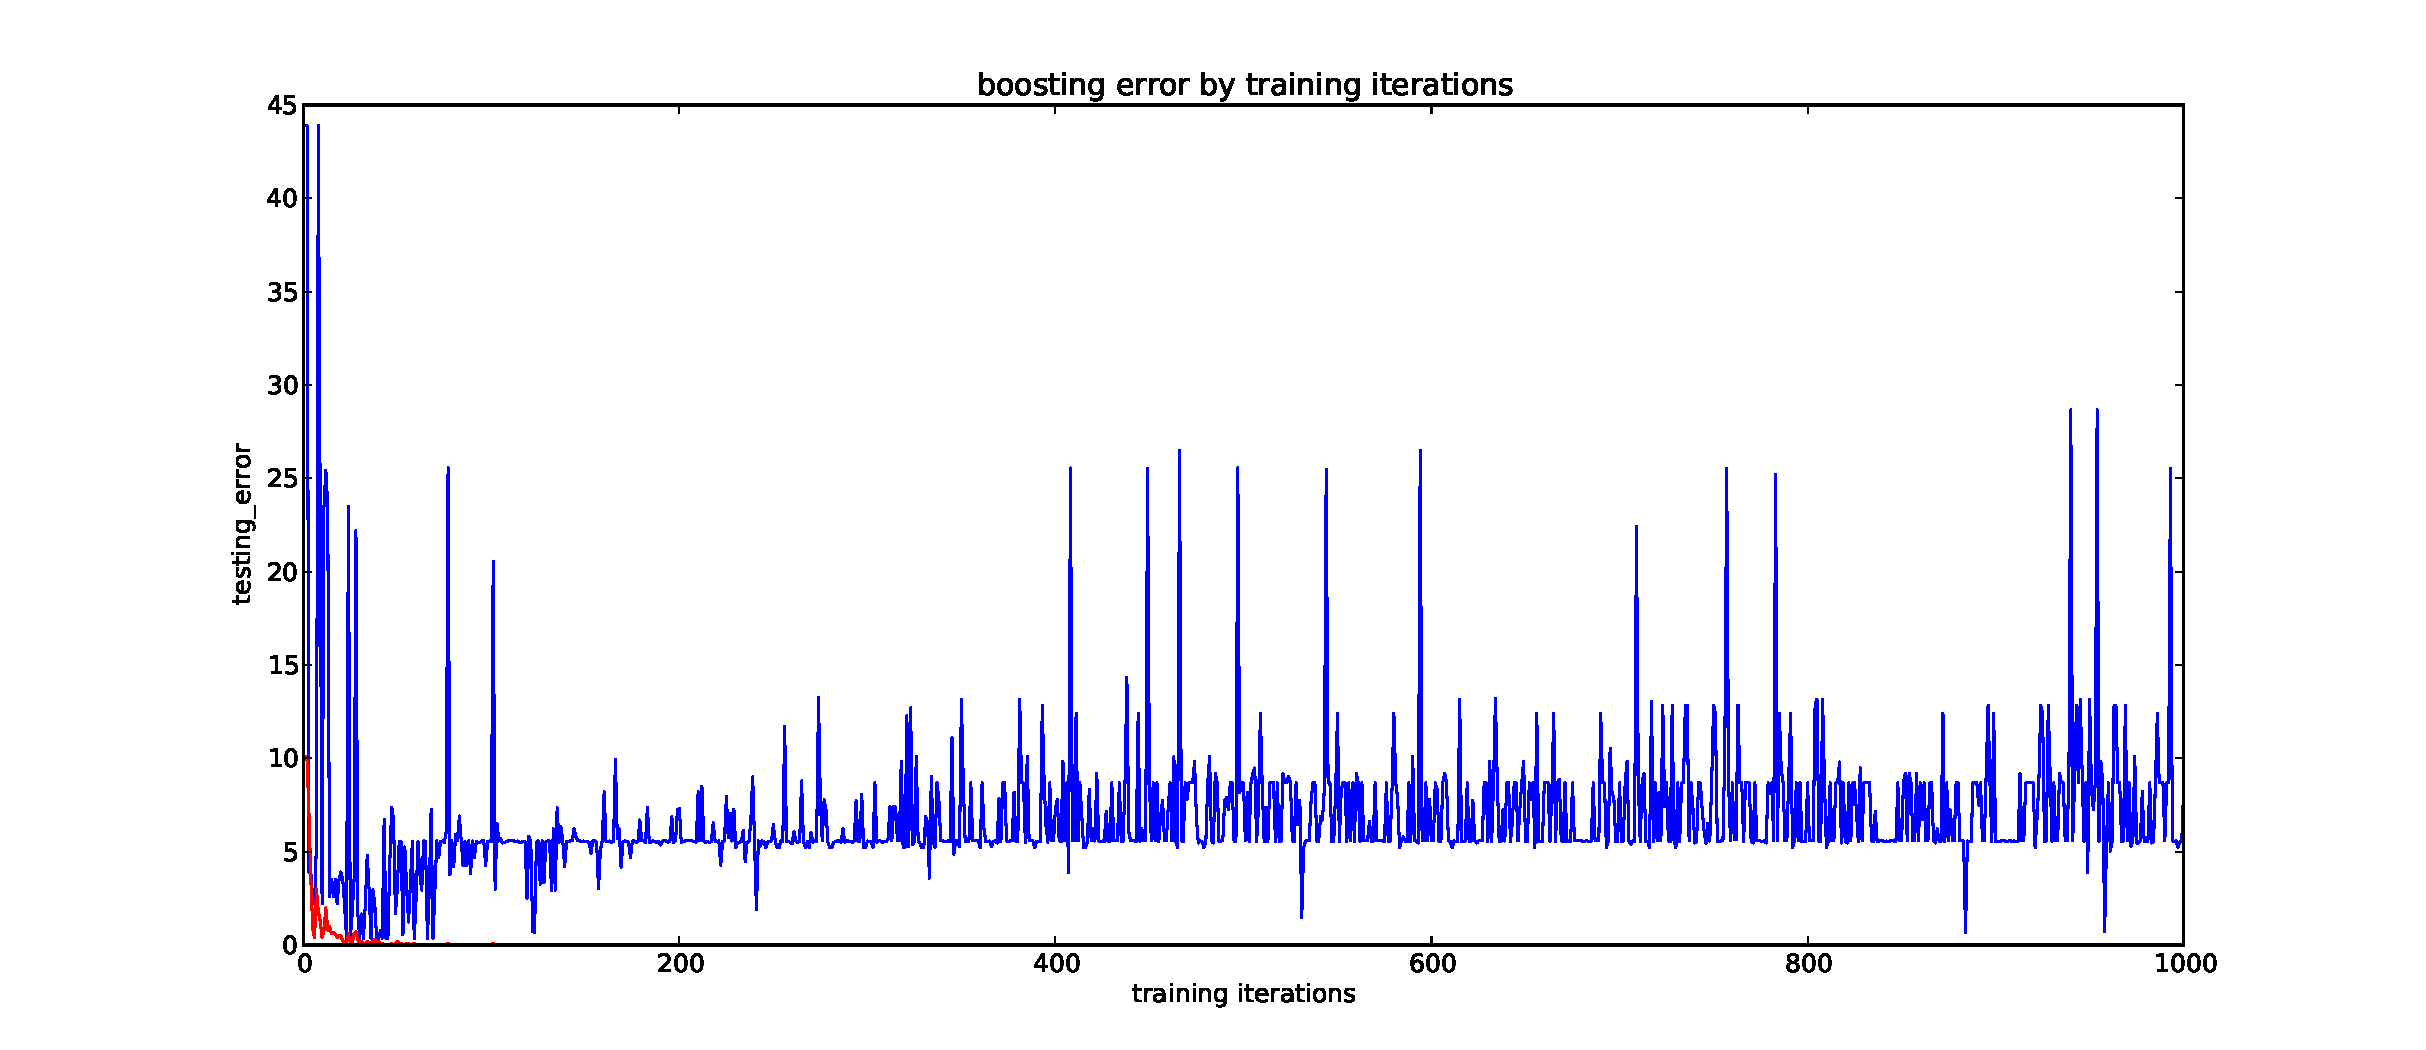
\includegraphics[width=3in]{data/agaricus-lepiota/boosting/training-iterations.pdf}
    \caption{Mushroom - error by boosting iterations \label{ag-boost-iter}}
\end{figure} 

An examination of the boosting behavior shows that, as expected, the odor attribute was chosen by the weak learner (decision stump), for many of the boosting iterations. Each time the instance weight distribution caused the learner to select a different attribute, the next iteration odor was again the attribute chosen.


\subsection{Support Vector Machines}
%You should implement (for sufficently loose definitions of implement including download) SVMs. This should be done in such a way that you can swap out kernel functions. I'd like to see at least two.

The SVM performance in the initial experiment performed well in regards to quickly converging to low classification error with just over 500 samples. This learner also performed quite consistently at the low test error rate as more training data was added. The SVM training times were the second highest, being consistently double to triple that of the other eager learners. It was still significantly faster than the neural network. Even after dropping the 63 nodes in the hidden layer, the neural network was still significantly slower than SVM at the same training set size.

Follow up experiments were performed to see how changes to the SVM kernel would affect it's performance. It can be seen from Figure~\ref{ag-svm-poly} that using a polynomial kernel function with degree 6 produced the smallest classification error (2\%), which is significantly lower than that achieved by the linear kernel (7\%).

\begin{figure}[!htbp]
    \centering
    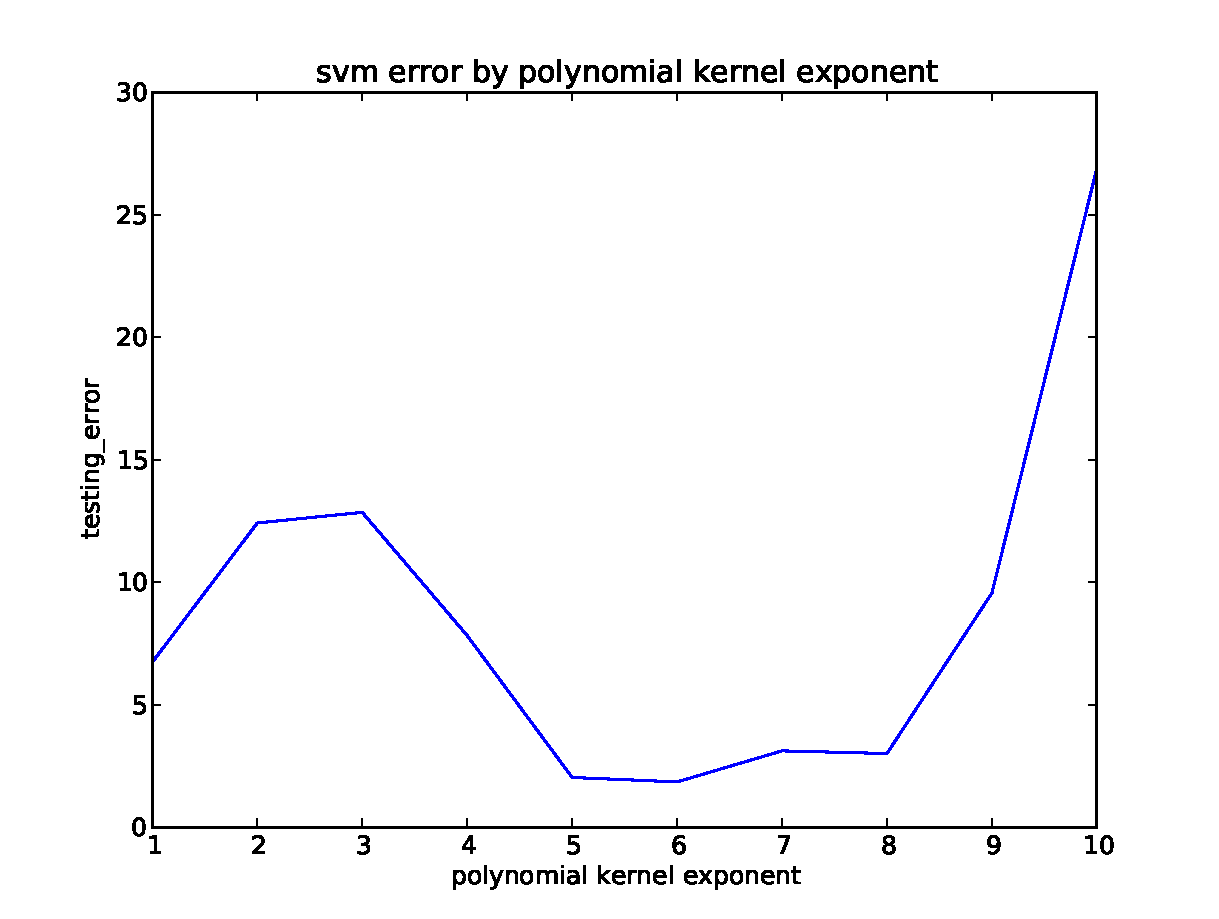
\includegraphics[width=3in]{data/agaricus-lepiota/svm/polynomial.pdf}
    \caption{Mushroom - error by svm polynomial kernel exponent \label{ag-svm-poly}}
\end{figure} 

The SVM kernel was then changed to a radial basis kernel to evaluate it's behavior. Figure~\ref{ag-svm-rbf} shows that the smallest classification error (2\%) was reached with a gamma of 0.225. This is the same error as that found using the degree 6 polynomial kernel. However, the RBF kernel took twice as long to train (0.8 sec vs. 0.4).

\begin{figure}[!htbp]
    \centering
    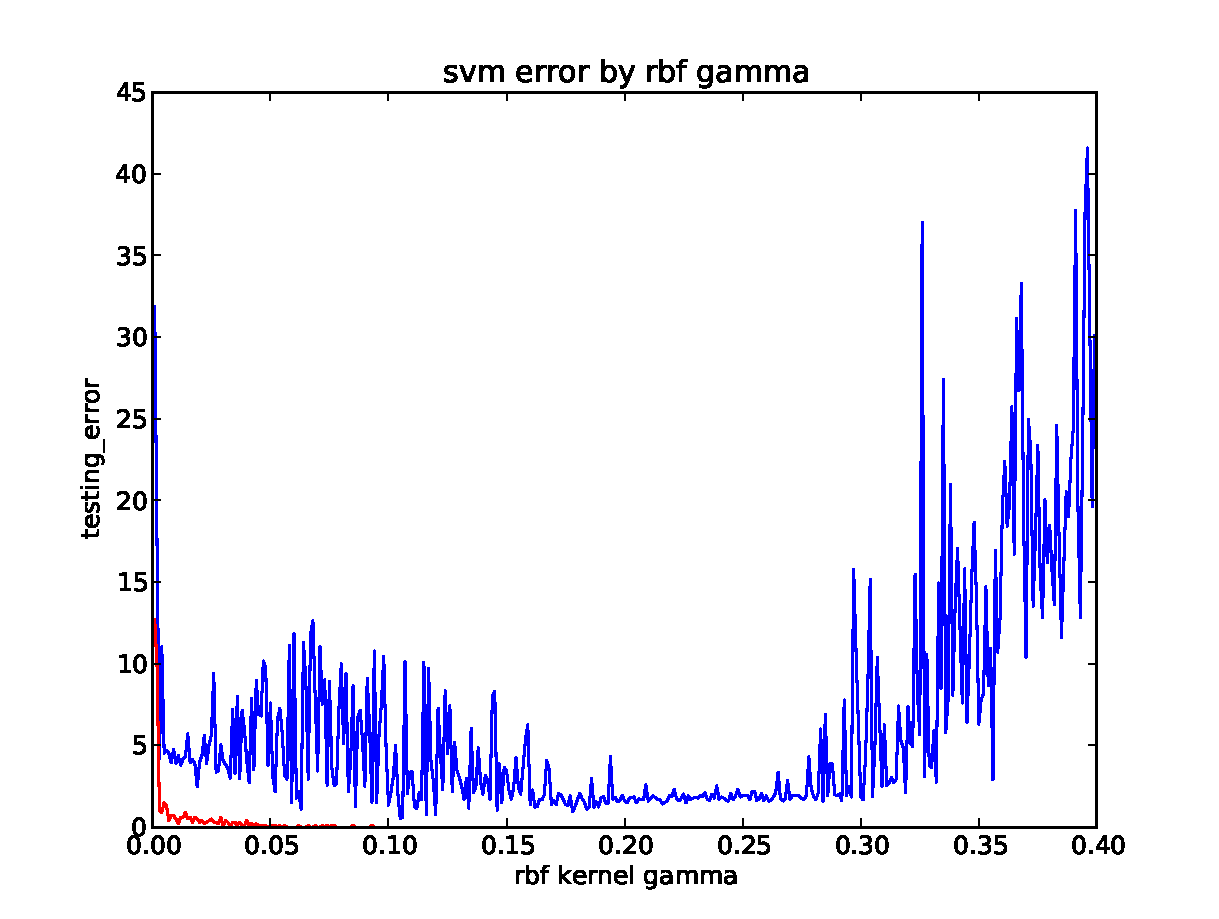
\includegraphics[width=3in]{data/agaricus-lepiota/svm/rbf.pdf}
    \caption{Mushroom - error by svm rbf gamma\label{ag-svm-rbf}}
\end{figure} 

\subsection{k-nearest neighbor}
%You should implement kNN. Use different values of k.

Initial performance results, with a single nearest neighbor, show a classification error of 3\%. Figure~\ref{ag-knn-k} shows the results of experimenting with various values for k. The plot indicates that k=3 lowered the error on a 1,000 instance training set to 2.5\%. 

\begin{figure}[!htbp]
    \centering
    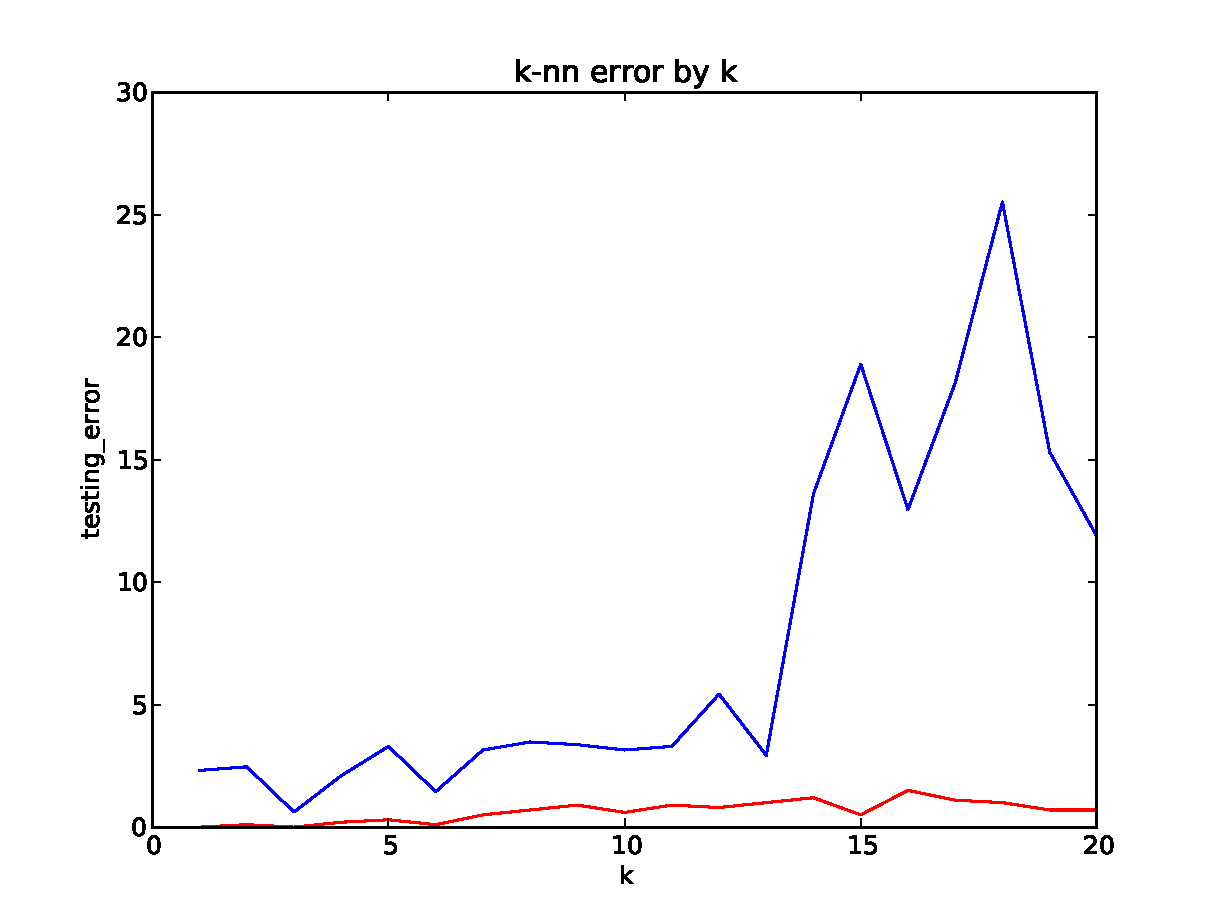
\includegraphics[width=3in]{data/agaricus-lepiota/k-nn/k.pdf}
    \caption{Mushroom - error by number of k-nn neighbors\label{ag-knn-k}}
\end{figure} 






\section{Classification - Income}

Our second dataset was also chosen from the UCI ML Repository and is titled, Adult \cite{Bache+Lichman:2013}. The classification task in this case is to determine if one's household income exeeds \$50,000/yr based on 14 biographical attributes. The data was collected from a census database from 1994. Attributes include the subject's age, level of education, marital-status, occupation, race, sex, etc. The full description of attributes can be found at http://archive.ics.uci.edu/ml/datasets/Adult.

\subsection{Attribute characteristics}

Value distributions for the income dataset are shown in Figure~\ref{ad-data-viz}. In this classification task, it is not as clear as before what attributes will contribute to correct classifications. Classes are fairly evenly distributed amongst the various attribute values. Some domain knowledge could help to make intuitive judgments. For example, individuals with high capital gains or losses would suppose greater net worth and likely greater income. Income could also correlate to one's occupation or education level.

Another difference with this dataset is that the two classifications are not as evenly distributed (76\% under 50k, 24\% over 50k). This will have implications when analyzing the performance of the various learners. The chosen metric will need to conform the use cases for the resulting model. For example, if the end user is most interested in correctly identifying all individuals with incomes greater than 50k, the performance metric should be the recall for that class. As can be seen in the example accuracy results from Figure~\ref{ad-metrics}, the classifier did well at positively identifying people making under 50k (0.95 true positive rate). However, it was only able to correctly identify 55\% of those making over 50k.

For the purposes of evaluating the current set of learners, the weighted average f-score (f-measure in Weka) was used. This provided a measure of both precision and recall metrics across both classifications. This will test each learner's ability to achieve a balanced confusion matrix.


\begin{figure}[!htbp]
    \centering
    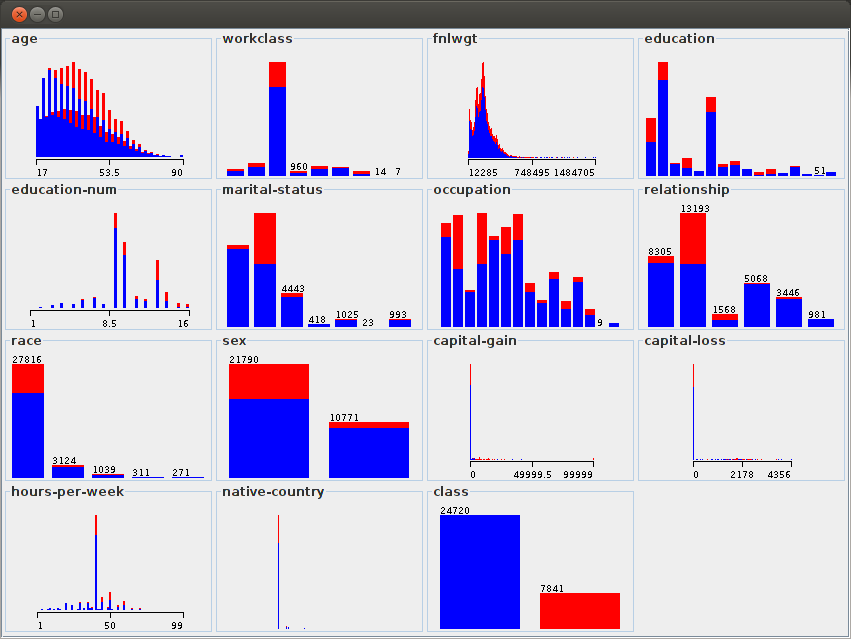
\includegraphics[width=3in]{data/adult/ad-data-viz.png}
    \caption{income attribute distribution and classification \label{ad-data-viz}}
\end{figure} 

\tiny
\begin{verbbox}

=== Detailed Accuracy By Class ===

               TP Rate   FP Rate   Precision   Recall  F-Measure   ROC Area  Class
                 0.952     0.449      0.873     0.952     0.911      0.865     <=50K
                 0.551     0.048      0.779     0.551     0.645      0.865     >50K
Weighted Avg.    0.858     0.355      0.851     0.858     0.849      0.865

=== Confusion Matrix ===

    a    b   <-- classified as
 8064  406 |    a =  <=50K
 1168 1433 |    b =  >50K

\end{verbbox}
\normalsize

\begin{figure}[!htbp]
    \centering
    \theverbbox
    \caption{example accuracy metrics for income \label{ad-metrics}}
\end{figure}


\subsubsection{Learning Curves}

\begin{figure}[!htbp]
    \centering
    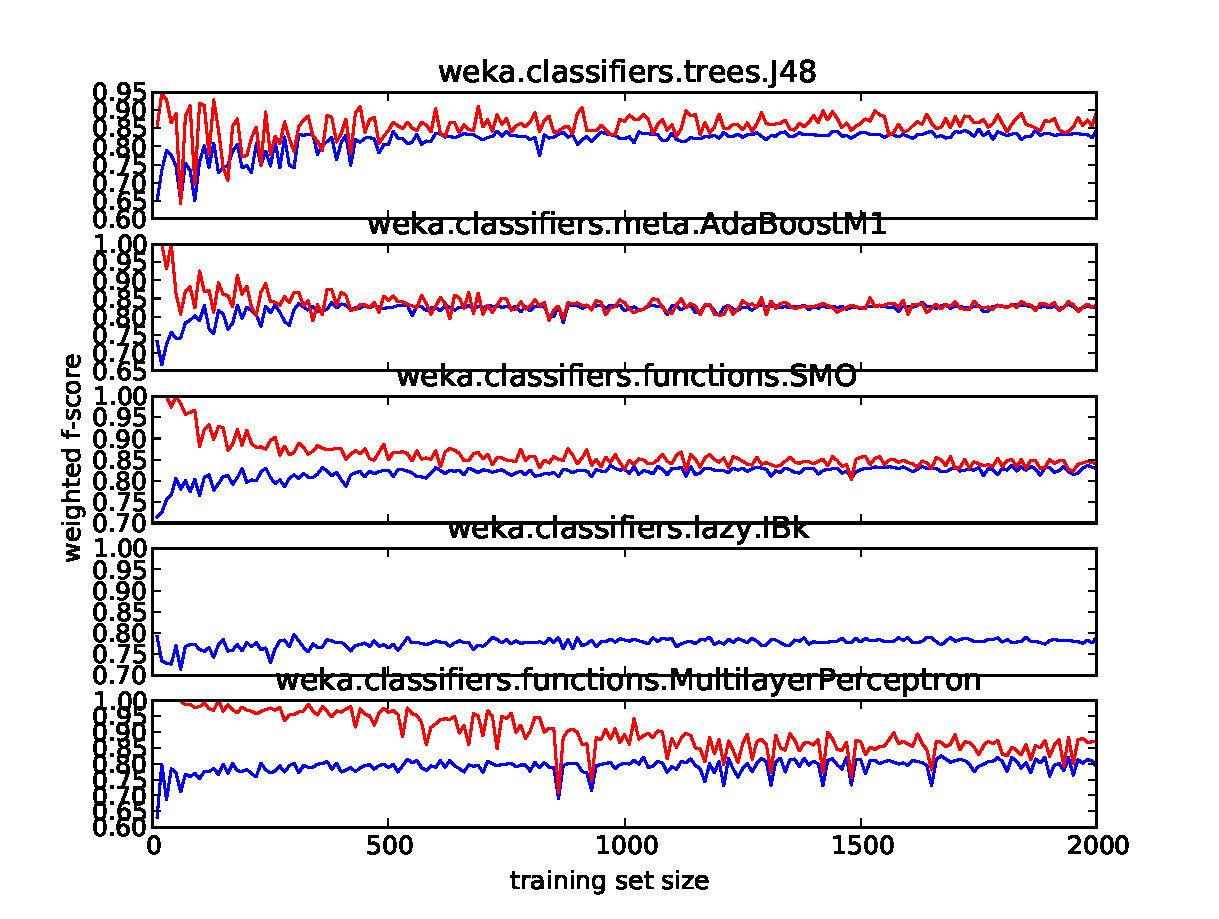
\includegraphics[width=3in]{data/adult/learning-curve-10to2000/stacked-fscore.pdf}
    \caption{Income - F-Score by Training Size \label{ad-error}}
\end{figure} 

\subsubsection{Training Times}

\begin{figure}[!htbp]
    \centering
    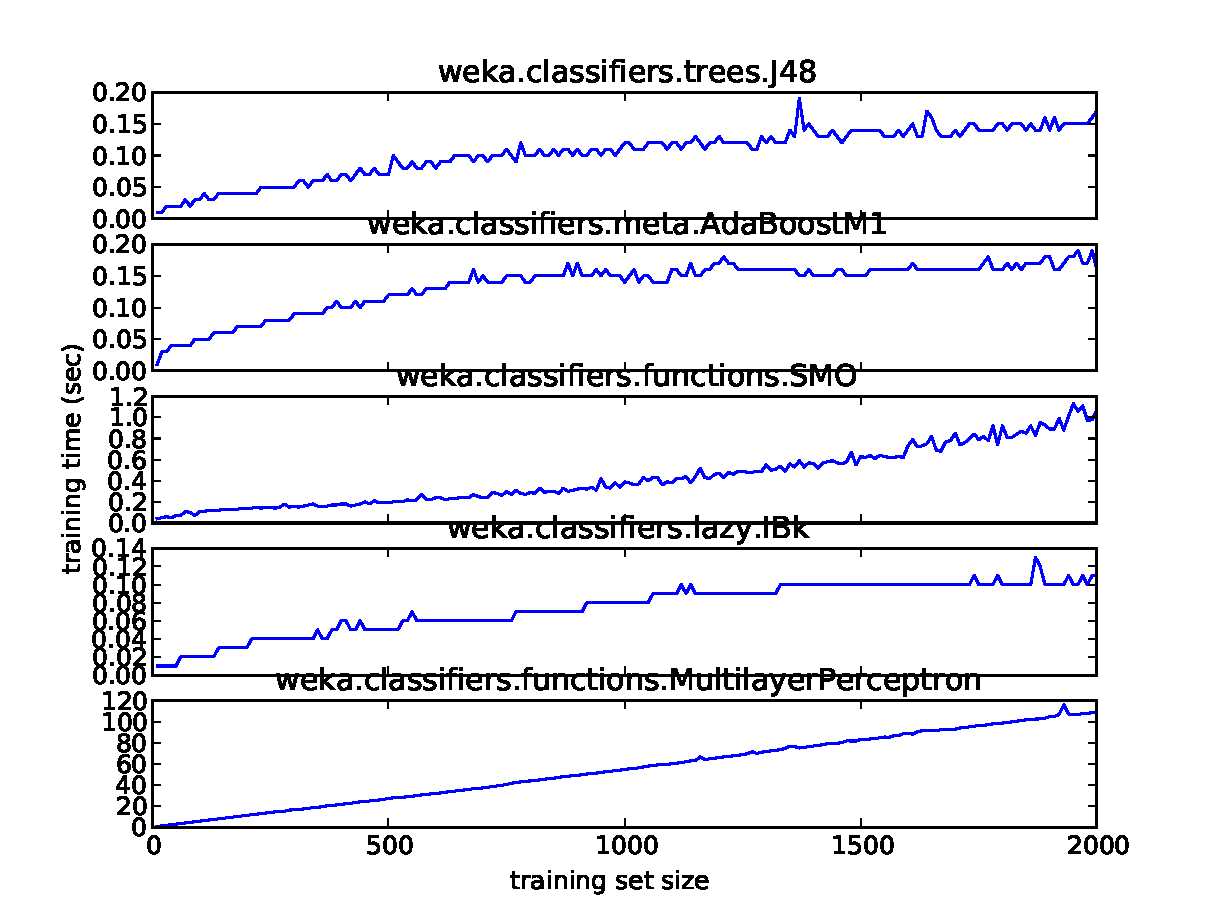
\includegraphics[width=3in]{data/adult/learning-curve-10to2000/runtime.pdf}
    \caption{Income - Training Time by Training Size \label{ad-runtime}}
\end{figure} 

\section{Analysis}

\subsection{Overview of Results}
%analyses of your results. Why did you get the results you did?

\subsection{Algorithm Comparison}
%Compare and contrast the different algorithms. What sort of changes might you make to each of those algorithms to improve performance? How fast were they in terms of wall clock time? Iterations? Would cross validation help (and if it would, why didn't you implement it?)? How much performance was due to the problems you chose? How about the values you chose for learning rates, stopping criteria, pruning methods, and so forth (and why doesn't your analysis show results for the different values you chose?)? Which algorithm performed best? How do you define best? Be creative and think of as many questions you can, and as many answers as you can.



\bibliographystyle{abbrv}
\bibliography{term-paper}
\begin{thebibliography}{10}

\bibitem{Bache+Lichman:2013}
K. Bache and M. Lichman
\newblock UCI Machine Learning Repository
\newblock 2013
\newblock http://archive.ics.uci.edu/ml
\newblock University of California, Irvine, School of Information and Computer Sciences

%\bibitem{Zhong:Osteo}
%L.~Zhong, D.~El-Daye, B.~Kaufman, N.~Tobaoda, T.~Mohamed, and M.~Liebschner.
%\newblock Osteoconduct: Wireless body-area communication based on bone
  %conduction.
%\newblock In {\em in Proc. Int. Conf. Body Area Networks (BodyNets)}, June
  %2007.

\end{thebibliography}
\end{document}
